\def\uf{Union-Find}
\def\null{\texttt{NULL}}
\def\makeset{$\mathop{makeset}(x)$}
\def\find{$\mathop{find}(x)$}
\def\union{$\mathop{union}(x, y)$}

\section{\uf}
\paragraph{Popis.}
Sú problémy, ktoré vyžadujú spájanie objektov do množín a množín navzájom 
a následné určovanie, do ktorej množiny objekt patrí. Od takejto \emph{
dátovej štruktúry pre disjunktné množiny} očakávame, že si bude udržiavať 
jednoznačného \emph{zástupcu} každej množiny a bude poskytovať 
tieto tri oprácie: 
\begin{itemize}
\item $\mathop{\mathbf{makeset}}(x)$ -- vytvorí novú množinu s jedným prvkom, 
ktorý nepatrí do žiadnej inej množiny;
\item $\mathop{\mathbf{find}}(x)$ -- nájde zástupcu množiny, v ktorej sa 
prvok $x$ nachádza;
\item $\mathop{\mathbf{union}}(x, y)$ -- vytvorí novú množinu, ktorá obsahuje 
všetky prvky v množinách, ktorých zástupcovia sú $x$ a $y$. Tieto 
množiny zmaže. Ďalej vyberie nového zástupcu novej množiny. Pre 
jednoduchosť, táto operácia predpokladá, že $x$ a $y$ sú 
zástupcovia množín.
\end{itemize}
Vďaka častej asociácií objektov a spájania množín ako vrcholy a hrany grafu 
sa často dátová štruktúra abstraktne reprezentuje ako 
\emph{les} -- množina zakorenených stromov. 
Konkrétnou implementáciou potom býva pole objektov -- vrcholov. Ku každému 
objektu sa musí udržiavať smerník $p(x)$ na otca v strome. Smerník zástupcu 
množiny ukazuje na hodnotu \null.

Operácia \makeset\ teda vytvorí nový prvok $x$ a nastaví $p(x) = \null$. 

Operáciu \find\ vykonáme tak, že budeme sledovať cestu po smerníkoch, až 
kým nenájdeme zástupcu. 

Operáciu \union\ ide najjednoduchšie vykonať tak, že presmerujeme smerník 
$p(y)$ na prvok $x$, teda $p(y) = x$. 
Môžeme ľahko pozorovať, že takýto \emph{naivný} spôsob je neefektívny, 
lebo nám operácia \find\ v najhoršom prípade, na $n$ prvkoch, trvá $O(n)$ 
krokov. 

\paragraph{Použitie.}
Vďaka dvom hlavným operáciam \find\ a \union\ 
je táto dátová štruktúra známejšia pod pojmom \emph{\uf}, ktorý 
používame aj my. Medzi najznámejšie problémy, ktoré sa riešia pomocou 
\uf\ patria Kruskalov algoritmus na nájdenie najlacnejšej kostry 
\citep{kruskal} a unifikácia \citep{unif}. Veľmi priamočiare použitie je 
na zodpovedanie otázky "Koľko je komponentov súvislosti?" alebo
"Sú dva prvky v rovnakej množine?" ("Sú dva objekty navzájom prepojené?"), 
ak máme dovolené za behu pridávať hrany (spájať množiny objektov). 
Niektoré ďalšie grafové problémy popísal napr. \citet{paths1}.



\paragraph{Heuristika na spájanie.}
Existujú dva prístupy ako zlepšiť operácie a tým aj zrýchliť ich vykonanie. 
Sú to: heuristika \emph{spájanie podľa ranku} a rôzne heuristiky na 
\emph{kompresiu cesty}. 

\begin{figure}
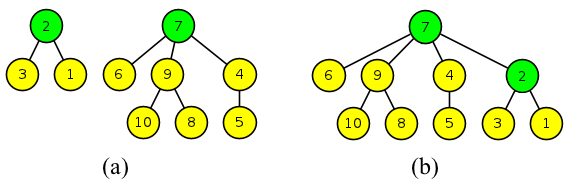
\includegraphics[width=\columnwidth]{obrazky/union.png}
\caption{\emph{Spájanie podľa ranku.} (a) Pred spojením. (b) Po spojení. 
Plytší strom sa napojil pod hlbší.} 
\label{img:union} 
\end{figure}

Prvá heuristika pridáva ku algoritmom hodnotu 
$rank(x)$, ktorá bude určovať najväčšiu možnú hĺbku podstromu zakorenenú 
vrcholom $x$. V tom prípade pri o\-pe\-rá\-cií \makeset\ zadefinujeme 
$rank(x) = 0$. 
Pri o\-pe\-rá\-cií \union\ vždy porovnáme $rank(x)$ a $rank(y)$, aby sme zistili, 
ktorý zástupca predstavuje menší strom. Smerník tohto zástupcu potom napojíme 
na zástupcu s výšším rankom. Zástupca novej množiny bude ten s vyšším rankom. 
Ak sú oba ranky rovnaké, vyberieme ľubovoľného zo zástupcov $x$ a $y$, 
jeho rank zvýšime o jeden a smerník ostatného zástupcu bude ukazovať 
na tohto zástupcu. Zástupcom novej množiny bude vybratý zástupca. 

\paragraph{Heuristiky na kompresiu cesty.}

\begin{figure}
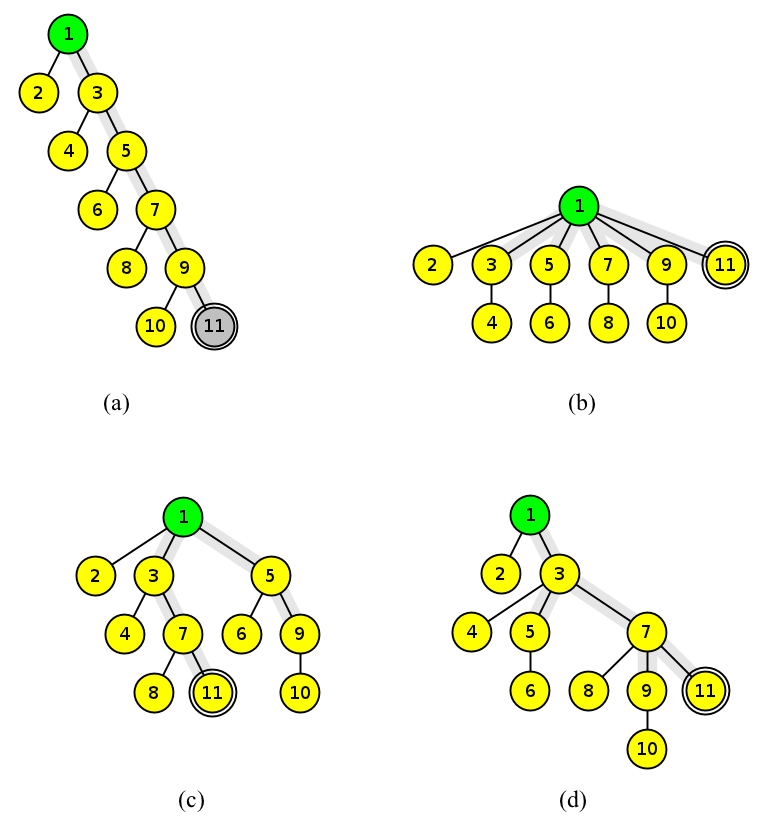
\includegraphics[width=\columnwidth]{obrazky/komp.png}
\caption{\emph{Kompresie cesty.} (a) Pred vykonaním \find. (b) Jednoduchá 
kompresia. (c) Delenie cesty. (d) Pólenie cesty.} 
\label{img:komp} 
\end{figure}

Druhou heuristikou je kompresia cesty. Algoritmov na efektívnu kompresiu 
cesty je veľa \citep{paths2}. Tu popíšeme tie najefektívnejšie. Prvou z nich 
je \emph{jednoduchá kompresia cesty} \citep{comp1}. Pri vykonávaní 
operácie \find, po tom, 
ako nájdeme zástupcu množiny obsahujúcej prvok $x$, smerníky prvkov 
navštívených po ceste (včetne $x$) presmerujeme na zástupcu množiny. Toto 
síce spomalí prvé vykonávanie, ale výrazne zrýchli ďalšie hľadania. 
Druhou heuristikou je \emph{delenie cesty} \citep{comp2}. Pri vykonávaní 
operácie \find\ 
pripojíme každý vrchol\footnote{Okrem koreňa a synov koreňa, 
keďže tie deda a otca resp. deda nemajú.} v ceste od vrcholu $x$ po koreň stromu 
na otca jeho otca. 
Treťou heuristikou je \emph{pólenie cesty} \citep{comp2}. Pri vykonávaní 
operácie \find\ 
pripojíme každý druhý vrchol\footnote{Okrem koreňa a synov koreňa, 
keďže tie deda a otca resp. deda nemajú.} 
v ceste od vrcholu $x$ po koreň stromu na otca jeho otca. 

Zdá sa, že najefektívnejšie je pólenie cesty pred delením, ktoré 
použije zhruba dvakrát viac priradení smerníkov a jednoduchou kompresiou, 
ktorá vyžaduje dva behy \citep{galil}. 

%citovat Walkerov alg. - to mám robiť tu?

